\section{Replicating the baseline model}\label{sec:baseline_model}

In this chapter, I describe the process of replicating and validating an existing model of vector-borne disease (VBD) spread. As outlined in the previous chapter, agent-based models (ABMs) are a suitable approach to representing VBD spread due to their ability to naturally incorporate individual-level heterogeneity and interventions. To benefit from the vast body of existing ABM VBD modelling literature, I base my work on an existing model that I extend with preventive measures and behaviour change theories. By employing an existing ABM, I ground my research using an accepted model within the field that lays the conceptual foundation for this project.

%The first task and contribution of this project is the replication of the selected baseline model.
The process of replicating the foundational ABM covered in this chapter provides confidence that the model functions as intended prior to further extensions and analysis. However, as outlined in the literature review, replicating ABMs from even well-defined ODD protocol descriptions can be challenging. Therefore, qualitative and quantitative comparisons of the results from the replicated model are necessary to ensure the correctness of the baseline model implementation across a range of scenarios. In the remainder of this chapter, I describe the chosen model to replicate and extend, along with the validation process to ensure the correctness of the ABM.

\subsection{Methods}

The model I chose as a foundation for this research is the hybrid ABM from \citet{manore_network-patch_2015}. The model builds on work by \citet{adams_man_2009} and \citet{perkins_heterogeneity_2013} to recreate a VBD outbreak, in which agents move about a network that spans different regions with distinct populations of mosquitoes. The dynamics of these mosquito populations are described by independent systems of ordinary differential equations (ODEs) that influence---and are influenced by---the agent-based component. Through the coupling of these two sub-models, VBD infection is spread through a combination of agent movement across regions and local mosquito population infection dynamics.

Many ABMs of VBD spread are designed to investigate specific entomological or epidemiological aspects of VBDs, which may limit their ability to generalise results if used as baseline models to incorporate preventive behaviours. For example, \citet{dommar_agent-based_2014} developed an ABM of chikungunya spread where mosquito populations were tied to precipitation estimates to investigate the timing and loci of disease spread. \citet{selvaraj_vector_2020} simulated malaria transmission to investigate evolutionary genetic mosquito resistance to insecticides. Incorporating preventive behaviours in such models may require behavioural processes to be designed around specific mechanisms that are not entirely relevant to this project. As an example, the focus on insecticide resistance in \citet{selvaraj_vector_2020} is arguably irrelevant to the main dynamics of preventive behaviours, and modelling this additional dimension may add unnecessary complexity to the model. Such precisely defined models may also present challenges during validation and parameterisation due to a lack of relevant data available.

Conversely, the model from \citet{manore_network-patch_2015} offers unique advantages due to its general formulation and part-ABM, part-ODE design. Originally proposed in \citet{mniszewski_towards_2014}, the equation-based patch sub-model draws on traditional VBD modelling literature to approximate mosquito population dynamics within regions (\textit{patches}) where mosquito populations are assumed to be well-mixed (often described as a \q{cloud} of mosquitoes). Patches in the model correspond to different geographical areas characterised by heterogeneous underlying environmental factors, and a network is overlaid on top of these patches which agents traverse according to an underlying movement model. Overall, this novel yet flexible approach offers a general framework for a VBD outbreak, and combined with the fact the model has previously been extended \cite{mateus_c_modeling_2021}, it is a well-suited foundation.

\subsubsection{Model description}\label{sec:baseline-model-description}

I used the Python programming language to replicate the baseline model from \citet{manore_network-patch_2015} due to the language's flexibility, abundant ecosystem for scientific computing, and external libraries for visualisation. Below, I follow the Overview, Design concepts, and Details (ODD) protocol \cite{grimm_standard_2006,grimm_odd_2020} to describe the model. To further aid replicability, I provide access to all code through a GitHub repository\footnote{\url{https://github.com/blademaw/mcs-project}}.

\odd{1. Purpose and patterns}

The purpose of the baseline model is to implement a computational representation of VBD spread through localised mosquito populations and network-wide agent mobility. The model from \citet{manore_network-patch_2015} produces an outbreak scenario of VBD spread with no re-infection mechanism, meaning the model is not equipped for endemic or steady-state prevalence dynamics. Specifically in this project, the model serves as a baseline to extend with features for preventive behaviours. The main pattern that served as a criterion for the model's utility in \citet{manore_network-patch_2015} was: \q{heterogeneity in mosquito habitat and host movement [altered] the dynamics of the initial spread and spatial patterns of a mosquito-borne disease.} This was investigated by varying mosquito densities in patches and simulating different agent movement tendencies.

\begin{figure}[h]
\centering

\definecolor{cf7f7f7}{RGB}{247,247,247}
\definecolor{cc9c9c9}{RGB}{201,201,201}
\definecolor{cdfdfdf}{RGB}{223,223,223}
\definecolor{cc1c1c1}{RGB}{193,193,193}
\definecolor{c0c1024}{RGB}{12,16,36}
\definecolor{c3ea44a}{RGB}{62,164,74}
\definecolor{c2e62b0}{RGB}{46,98,176}
\definecolor{c35479c}{RGB}{53,71,156}
\definecolor{cbb7ee4}{RGB}{187,126,228}
\definecolor{c5a71fa}{RGB}{90,113,250}
\definecolor{cefef2e}{RGB}{239,239,46}
\definecolor{c14c50f}{RGB}{20,197,15}


\def \globalscale {1.000000}
\begin{tikzpicture}[y=1cm, x=1cm, yscale=\globalscale,xscale=\globalscale, every node/.append style={scale=\globalscale}, inner sep=0pt, outer sep=0pt]
  \path[draw=black,fill=cf7f7f7,even odd rule,line width=0.05cm] (3.3108, 14.2989) rectangle (6.5472, 8.0599);



  \path[draw=cc9c9c9,fill=white,even odd rule,line width=0.0516cm] (11.9826, 14.3339) rectangle (15.4091, 8.0581);



  \path[draw=black,fill=cdfdfdf,even odd rule,line width=0.05cm] (7.2484, 14.3349) rectangle (11.6176, 11.2963);



  \path[draw=black,fill=cc1c1c1,even odd rule,line width=0.05cm] (7.2664, 10.7569) rectangle (11.6176, 8.0599);



  \node[text=black,even odd rule,line width=0.0204cm,anchor=south west,scale=.85] (text23) at (3.355, 8.1608){$k=1$};



  \node[text=black,even odd rule,line width=0.0204cm,anchor=south west] (text23-8) at (12.1931, 13.4883){\textbf{Activities}};



  \node[text=black,even odd rule,line width=0.0204cm,anchor=south west,scale=.85] (text23-5) at (10.7, 8.1279){$k=3$};



  \node[text=black,even odd rule,line width=0.0204cm,anchor=south west,scale=.85] (text23-5-7) at (10.7, 11.3661){$k=2$};



  \node[text=black,even odd rule,line width=0.0204cm,anchor=south west] (text23-5-7-4) at (13.1675, 12.3933){Home};



  \node[text=black,even odd rule,line width=0.0204cm,anchor=south west] (text23-5-7-4-1) at (13.1611, 11.3729){Work};



  \begin{scope}[shift={(-0.7673, -2.3626)}]
    \node[text=black,even odd rule,line width=0.0204cm,anchor=south west] (text23-5-7-4-4) at (13.9321, 12.7){Shopping};



    \node[text=black,even odd rule,line width=0.0204cm,anchor=south west] (text23-5-7-4-4-8) at (13.9315, 11.7081){Recreation};



  \end{scope}
  \begin{scope}[draw=c0c1024,line cap=,line join=miter,line width=0.0369cm,cm={ 1.0333,-0.0,-0.0,-1.6099,(-0.1338, 32.7062)}]
    \path[draw=c0c1024,line cap=,line join=miter,line width=0.0369cm] (8.263, 12.4514) -- (9.7002, 12.8683);



    \path[draw=c0c1024,line cap=,line join=miter,line width=0.0369cm] (8.2433, 12.4514) -- (10.0546, 11.9459);



    \path[draw=c0c1024,line cap=,line join=miter,line width=0.0369cm] (7.8693, 14.5614) -- (5.2902, 14.6752);



    \path[draw=c0c1024,line cap=,line join=miter,line width=0.0369cm] (5.2705, 12.0597) -- (9.3852, 14.0939);



    \path[draw=c0c1024,line cap=,line join=miter,line width=0.0369cm] (7.889, 14.5614) -- (5.3296, 12.047);



    \path[draw=c0c1024,line cap=,line join=miter,line width=0.0369cm] (4.4593, 13.2515) -- (5.2875, 14.6497);



    \path[draw=c0c1024,line cap=,line join=miter,line width=0.0369cm] (5.2875, 12.0612) -- (5.3235, 14.6613);



    \path[draw=c0c1024,line cap=,line join=miter,line width=0.0369cm] (4.4773, 13.2284) -- (9.3927, 14.095);



    \path[draw=c0c1024,line cap=,line join=miter,line width=0.0369cm] (7.8443, 14.5688) -- (9.4287, 14.095);



    \path[draw=c0c1024,line cap=,line join=miter,line width=0.0369cm] (7.9163, 14.5573) -- (8.2584, 12.4541);



    \path[draw=c0c1024,line cap=,line join=miter,line width=0.0369cm] (7.8803, 14.5688) -- (10.0769, 11.9457);



    \path[draw=c0c1024,line cap=,line join=miter,line width=0.0369cm] (9.7528, 12.8586) -- (10.0229, 11.9457);



    \path[draw=c0c1024,line cap=,line join=miter,line width=0.0369cm] (5.2875, 12.0497) -- (10.0769, 11.9341);



    \path[fill=c3ea44a,nonzero rule,line cap=,line join=miter,line width=0.0004cm] (11.0475, 14.1075).. controls (11.0915, 14.2163) and (11.0435, 14.3347) .. (11.0428, 14.3365).. controls (11.0429, 14.3359) and (11.044, 14.3274) .. (11.044, 14.3274).. controls (11.0581, 14.2543) and (11.0238, 14.2131) .. (11.0238, 14.2131).. controls (11.0469, 14.2764) and (11.0042, 14.3124) .. (10.9791, 14.3274).. controls (10.9697, 14.3331) and (10.9627, 14.3379) .. (10.9627, 14.3379).. controls (10.962, 14.3379) and (10.9613, 14.3303) .. (10.9608, 14.3274).. controls (10.9439, 14.2382) and (11.0237, 14.1245) .. (11.0237, 14.1245).. controls (10.9727, 14.1536) and (10.9417, 14.2485) .. (10.9281, 14.3006).. controls (10.9443, 14.2127) and (10.9175, 14.1722) .. (10.9175, 14.1722).. controls (10.9281, 14.2457) and (10.9015, 14.3061) .. (10.8903, 14.3274).. controls (10.8875, 14.3328) and (10.8857, 14.3379) .. (10.8857, 14.3379).. controls (10.8843, 14.3379) and (10.8832, 14.3305) .. (10.8821, 14.3274).. controls (10.8629, 14.2743) and (10.8724, 14.1432) .. (10.8724, 14.1432).. controls (10.8533, 14.1738) and (10.8419, 14.2366) .. (10.8358, 14.2822).. controls (10.8358, 14.2049) and (10.798, 14.1586) .. (10.798, 14.1586).. controls (10.8379, 14.2574) and (10.7848, 14.3222) .. (10.7848, 14.3222).. controls (10.7954, 14.2336) and (10.7582, 14.2114) .. (10.7582, 14.2114).. controls (10.7857, 14.2481) and (10.7237, 14.3205) .. (10.7237, 14.3205).. controls (10.6998, 14.2251) and (10.7582, 14.0904) .. (10.7582, 14.0904).. controls (10.7228, 14.1224) and (10.7021, 14.2025) .. (10.6912, 14.2607).. controls (10.69, 14.1867) and (10.6419, 14.1586) .. (10.6419, 14.1586).. controls (10.6903, 14.2336) and (10.6414, 14.3256) .. (10.6414, 14.3256).. controls (10.6467, 14.237) and (10.6121, 14.1944) .. (10.6121, 14.1944).. controls (10.6165, 14.2335) and (10.5674, 14.3034) .. (10.5495, 14.3274).. controls (10.5456, 14.3327) and (10.5431, 14.3378) .. (10.5431, 14.3378).. controls (10.5421, 14.3378) and (10.5412, 14.3304) .. (10.5404, 14.3274).. controls (10.5226, 14.2616) and (10.559, 14.1211) .. (10.559, 14.1211).. controls (10.5172, 14.1419) and (10.4917, 14.2903) .. (10.4859, 14.3274).. controls (10.4851, 14.3328) and (10.4847, 14.3379) .. (10.4847, 14.3379).. controls (10.4844, 14.3379) and (10.4842, 14.3303) .. (10.4839, 14.3274).. controls (10.4784, 14.2698) and (10.479, 14.2059) .. (10.479, 14.2059).. controls (10.4614, 14.2183) and (10.4476, 14.3378) .. (10.4475, 14.3378) -- (10.448, 14.3274).. controls (10.4594, 14.1785) and (10.4183, 14.1296) .. (10.4183, 14.1296).. controls (10.4384, 14.2028) and (10.4021, 14.2988) .. (10.3901, 14.3274).. controls (10.3878, 14.3328) and (10.3864, 14.3378) .. (10.3864, 14.3378).. controls (10.3838, 14.3378) and (10.3815, 14.3305) .. (10.3796, 14.3274).. controls (10.3517, 14.2835) and (10.3864, 14.1824) .. (10.3864, 14.1824).. controls (10.3544, 14.2089) and (10.3434, 14.2556) .. (10.3398, 14.2905).. controls (10.3428, 14.1114) and (10.32, 14.0529) .. (10.32, 14.0529).. controls (10.3364, 14.1175) and (10.3013, 14.2878) .. (10.2927, 14.3274).. controls (10.2922, 14.3298) and (10.2922, 14.3295) .. (10.2927, 14.3274) -- (10.292, 14.3274).. controls (10.2983, 14.2671) and (10.2669, 14.1586) .. (10.2669, 14.1586).. controls (10.2669, 14.2059) and (10.25, 14.2991) .. (10.2446, 14.3274).. controls (10.2436, 14.3328) and (10.243, 14.3378) .. (10.243, 14.3378).. controls (10.2403, 14.3344) and (10.239, 14.3303) .. (10.2372, 14.3274).. controls (10.1967, 14.2503) and (10.243, 14.1211) .. (10.243, 14.1211).. controls (10.1814, 14.1739) and (10.1747, 14.2947) .. (10.1741, 14.3274).. controls (10.174, 14.3299) and (10.174, 14.3306) .. (10.1741, 14.3274).. controls (10.1741, 14.3274) and (10.1772, 14.34) .. (10.1686, 14.3274).. controls (10.139, 14.2863) and (10.1757, 14.1586) .. (10.1757, 14.1586).. controls (10.1393, 14.1834) and (10.1245, 14.2958) .. (10.1212, 14.3274).. controls (10.1207, 14.3327) and (10.12, 14.3378) .. (10.12, 14.3378).. controls (10.1191, 14.3378) and (10.1181, 14.3302) .. (10.1174, 14.3274).. controls (10.0885, 14.2187) and (10.1741, 14.0982) .. (10.1741, 14.0982).. controls (10.0892, 14.1323) and (10.0672, 14.3378) .. (10.0672, 14.3378) -- (10.0672, 14.4316) -- (11.1059, 14.4316) -- (11.1059, 14.3274) -- (11.1059, 14.3274).. controls (11.106, 14.1367) and (11.0475, 14.1075) .. (11.0475, 14.1075) -- cycle;



    \path[fill=c2e62b0,line cap=,line join=miter,line width=0.0001cm] (10.419, 14.3237).. controls (10.6757, 14.3371) and (10.846, 14.3521) .. (10.9648, 14.3716).. controls (11.0442, 14.3847) and (11.1008, 14.4015) .. (11.1248, 14.4192).. controls (11.1346, 14.4266) and (11.1419, 14.4372) .. (11.1432, 14.4459).. controls (11.1438, 14.452) and (11.1432, 14.4547) .. (11.1392, 14.4615).. controls (11.1303, 14.4774) and (11.1125, 14.4885) .. (11.0776, 14.5).. controls (11.0246, 14.5175) and (10.9605, 14.5303) .. (10.7474, 14.5658).. controls (10.5341, 14.6014) and (10.4506, 14.6208) .. (10.42, 14.6418).. controls (10.4102, 14.6485) and (10.4106, 14.6496) .. (10.4241, 14.656).. controls (10.4464, 14.6665) and (10.4907, 14.6771) .. (10.6023, 14.6985).. controls (10.7143, 14.72) and (10.7673, 14.732) .. (10.8056, 14.7442).. controls (10.8498, 14.7583) and (10.8736, 14.7713) .. (10.8866, 14.7882).. controls (10.8909, 14.7937) and (10.8914, 14.7957) .. (10.8916, 14.8059).. controls (10.8916, 14.8172) and (10.8915, 14.8175) .. (10.8839, 14.8274).. controls (10.8777, 14.8352) and (10.8731, 14.8394) .. (10.8608, 14.8474).. controls (10.8423, 14.8592) and (10.8248, 14.8669) .. (10.7937, 14.8766).. controls (10.7408, 14.8931) and (10.684, 14.9036) .. (10.5213, 14.9269).. controls (10.3269, 14.9546) and (10.2386, 14.9717) .. (10.1544, 14.9977).. controls (10.0668, 15.0247) and (10.012, 15.0531) .. (9.9641, 15.0965).. controls (9.9465, 15.1124) and (9.9185, 15.1316) .. (9.8956, 15.1434).. controls (9.8486, 15.1675) and (9.7793, 15.1902) .. (9.7024, 15.207).. controls (9.6098, 15.2271) and (9.5014, 15.2413) .. (9.3962, 15.247) -- (9.3802, 15.2479) -- (9.406, 15.2485).. controls (9.4202, 15.2488) and (9.372, 15.2493) .. (9.2988, 15.2494).. controls (9.2171, 15.2495) and (9.1628, 15.2492) .. (9.1582, 15.2485).. controls (9.1539, 15.2479) and (9.1397, 15.2466) .. (9.1265, 15.2456).. controls (9.0435, 15.2394) and (8.9661, 15.2236) .. (8.9239, 15.2043).. controls (8.8532, 15.1721) and (8.8456, 15.1277) .. (8.9016, 15.0769).. controls (8.9162, 15.0638) and (8.9592, 15.0361) .. (8.9823, 15.025).. controls (9.0774, 14.9794) and (9.2091, 14.9439) .. (9.406, 14.9109).. controls (9.4833, 14.898) and (9.5634, 14.8867) .. (9.7344, 14.8646).. controls (9.9157, 14.8413) and (9.9353, 14.8386) .. (9.9837, 14.8307).. controls (10.0446, 14.8208) and (10.0892, 14.8098) .. (10.1015, 14.8015).. controls (10.1047, 14.7995) and (10.1085, 14.7959) .. (10.1099, 14.7938).. controls (10.1122, 14.7901) and (10.1122, 14.7893) .. (10.1098, 14.786).. controls (10.1012, 14.7746) and (10.0622, 14.7642) .. (9.9622, 14.7465).. controls (9.8545, 14.7273) and (9.8162, 14.718) .. (9.7866, 14.7037).. controls (9.7585, 14.6901) and (9.7485, 14.6714) .. (9.7594, 14.6524).. controls (9.7781, 14.6201) and (9.8484, 14.5951) .. (9.9971, 14.5677).. controls (10.0848, 14.5515) and (10.166, 14.5398) .. (10.3852, 14.5114).. controls (10.5511, 14.49) and (10.5999, 14.4833) .. (10.6504, 14.4753).. controls (10.7359, 14.4619) and (10.7827, 14.4504) .. (10.7916, 14.4409).. controls (10.8026, 14.4288) and (10.7855, 14.4166) .. (10.7371, 14.4019).. controls (10.6707, 14.3817) and (10.5438, 14.362) .. (10.3887, 14.3481).. controls (10.3736, 14.3467) and (10.3585, 14.345) .. (10.3553, 14.3441).. controls (10.3433, 14.341) and (10.3414, 14.3283) .. (10.3522, 14.3237).. controls (10.3576, 14.3214) and (10.3761, 14.3214) .. (10.419, 14.3237) -- cycle;



    \begin{scope}[fill=c3ea44a,line cap=,line join=miter,line width=0.0369cm,cm={ 0.0137,-0.0,-0.0,-0.0088,(8.6487, 14.888)}]
      \begin{scope}[fill=c3ea44a,line cap=,line join=miter,line width=0.0369cm]
        \begin{scope}[fill=c3ea44a,line cap=,line join=miter,line width=0.0369cm]
          \path[fill=c3ea44a,line cap=,line join=miter,line width=0.0369cm] (71.6354, -6.7299).. controls (74.8473, -19.1172) and (71.3405, -32.6025) .. (71.2912, -32.8101).. controls (71.3, -32.7443) and (71.3785, -31.7753) .. (71.3785, -31.7753).. controls (72.4083, -23.4539) and (69.8984, -18.7605) .. (69.8984, -18.7605).. controls (71.5924, -25.9599) and (68.4665, -30.0649) .. (66.6333, -31.7753).. controls (65.9465, -32.4154) and (65.4353, -32.9619) .. (65.4353, -32.9619).. controls (65.3822, -32.9619) and (65.3354, -32.0979) .. (65.2961, -31.7753).. controls (64.0641, -21.6145) and (69.8971, -8.6719) .. (69.8971, -8.6719).. controls (66.1651, -11.9888) and (63.9045, -22.7833) .. (62.9102, -28.7226).. controls (64.0957, -18.7136) and (62.1361, -14.1039) .. (62.1361, -14.1039).. controls (62.9102, -22.4746) and (60.9658, -29.3451) .. (60.1498, -31.7753).. controls (59.9449, -32.3875) and (59.8083, -32.9619) .. (59.8083, -32.9619).. controls (59.7134, -32.9619) and (59.6287, -32.1232) .. (59.5477, -31.7753).. controls (58.146, -25.7246) and (58.838, -10.8047) .. (58.838, -10.8047).. controls (57.4465, -14.2849) and (56.6089, -21.436) .. (56.1613, -26.6266).. controls (56.1639, -17.827) and (53.4047, -12.5505) .. (53.4047, -12.5505).. controls (56.3156, -23.8043) and (52.4345, -31.1769) .. (52.4345, -31.1769).. controls (53.2098, -21.0882) and (50.4939, -18.5658) .. (50.4939, -18.5658).. controls (52.5002, -22.7416) and (47.9715, -30.9847) .. (47.9715, -30.9847).. controls (46.2258, -20.1193) and (50.4939, -4.7895) .. (50.4939, -4.7895).. controls (47.9094, -8.4315) and (46.3926, -17.5474) .. (45.5982, -24.175).. controls (45.5134, -15.7561) and (41.9978, -12.5505) .. (41.9978, -12.5505).. controls (45.5311, -21.0882) and (41.9572, -31.5653) .. (41.9572, -31.5653).. controls (42.3458, -21.4765) and (39.8219, -16.6239) .. (39.8219, -16.6239).. controls (40.1393, -21.0782) and (36.5491, -29.0441) .. (35.2437, -31.7741).. controls (34.9565, -32.3724) and (34.7768, -32.9607) .. (34.7768, -32.9607).. controls (34.7022, -32.9607) and (34.639, -32.1093) .. (34.5808, -31.7741).. controls (33.2765, -24.28) and (35.9407, -8.2811) .. (35.9407, -8.2811).. controls (32.8869, -10.6568) and (31.0197, -27.5527) .. (30.5984, -31.7754).. controls (30.5377, -32.3839) and (30.5074, -32.9621) .. (30.5074, -32.9621).. controls (30.4897, -32.9621) and (30.4694, -32.0967) .. (30.4505, -31.7754).. controls (30.0482, -25.2162) and (30.0925, -17.9384) .. (30.0925, -17.9384).. controls (28.8085, -19.3477) and (27.7965, -32.9607) .. (27.7901, -32.9607) -- (27.8242, -31.7741).. controls (28.6591, -14.8238) and (25.656, -9.2526) .. (25.656, -9.2526).. controls (27.1259, -17.5804) and (24.4718, -28.5192) .. (23.5965, -31.7741).. controls (23.432, -32.3876) and (23.3283, -32.9607) .. (23.3283, -32.9607).. controls (23.136, -32.9607) and (22.9715, -32.127) .. (22.8273, -31.7741).. controls (20.7894, -26.7773) and (23.3283, -15.2666) .. (23.3283, -15.2666).. controls (20.9854, -18.2774) and (20.1847, -23.593) .. (19.9241, -27.5716).. controls (20.1392, -7.1829) and (18.4769, -0.52) .. (18.4769, -0.52).. controls (19.6724, -7.8724) and (17.1044, -27.2629) .. (16.4769, -31.7741).. controls (16.4403, -32.0399) and (16.444, -32.0119) .. (16.4769, -31.7741) -- (16.4264, -31.7741).. controls (16.8906, -24.91) and (14.5959, -12.5505) .. (14.5959, -12.5505).. controls (14.5959, -17.9384) and (13.3587, -28.547) .. (12.9678, -31.7741).. controls (12.8943, -32.3813) and (12.8502, -32.9607) .. (12.8502, -32.9607).. controls (12.6516, -32.5648) and (12.5554, -32.1006) .. (12.4238, -31.7741).. controls (9.4673, -22.9908) and (12.8502, -8.2811) .. (12.8502, -8.2811).. controls (8.3443, -14.2899) and (7.8572, -28.0458) .. (7.8104, -31.7739).. controls (7.8065, -32.0611) and (7.8053, -32.1396) .. (7.8104, -31.7739).. controls (7.8104, -31.7739) and (8.0406, -33.201) .. (7.4094, -31.7739).. controls (5.245, -27.097) and (7.9293, -12.5504) .. (7.9293, -12.5504).. controls (5.2701, -15.3765) and (4.1886, -28.1698) .. (3.9496, -31.7739).. controls (3.9104, -32.3748) and (3.8611, -32.9606) .. (3.8611, -32.9606).. controls (3.7952, -32.9606) and (3.7232, -32.0941) .. (3.6687, -31.7739).. controls (1.5573, -19.393) and (7.8142, -5.6799) .. (7.8142, -5.6799).. controls (1.6067, -9.5611) and (0.0, -32.9593) .. (0.0, -32.9593) -- (0.0, -43.6326) -- (75.9023, -43.6326) -- (75.9023, -31.7739) -- (75.9023, -31.7739).. controls (75.9137, -10.0558) and (71.6354, -6.7299) .. (71.6354, -6.7299) -- cycle;



        \end{scope}
      \end{scope}
    \end{scope}
    \begin{scope}[fill=c3ea44a,line cap=,line join=miter,line width=0.0369cm,cm={ 0.0137,-0.0,-0.0,-0.0088,(9.3372, 14.8826)}]
      \begin{scope}[fill=c3ea44a,line cap=,line join=miter,line width=0.0369cm]
        \begin{scope}[fill=c3ea44a,line cap=,line join=miter,line width=0.0369cm]
          \path[fill=c3ea44a,line cap=,line join=miter,line width=0.0369cm] (71.6354, -6.7299).. controls (74.8473, -19.1172) and (71.3405, -32.6025) .. (71.2912, -32.8101).. controls (71.3, -32.7443) and (71.3785, -31.7753) .. (71.3785, -31.7753).. controls (72.4083, -23.4539) and (69.8984, -18.7605) .. (69.8984, -18.7605).. controls (71.5924, -25.9599) and (68.4665, -30.0649) .. (66.6333, -31.7753).. controls (65.9465, -32.4154) and (65.4353, -32.9619) .. (65.4353, -32.9619).. controls (65.3822, -32.9619) and (65.3354, -32.0979) .. (65.2961, -31.7753).. controls (64.0641, -21.6145) and (69.8971, -8.6719) .. (69.8971, -8.6719).. controls (66.1651, -11.9888) and (63.9045, -22.7833) .. (62.9102, -28.7226).. controls (64.0957, -18.7136) and (62.1361, -14.1039) .. (62.1361, -14.1039).. controls (62.9102, -22.4746) and (60.9658, -29.3451) .. (60.1498, -31.7753).. controls (59.9449, -32.3875) and (59.8083, -32.9619) .. (59.8083, -32.9619).. controls (59.7134, -32.9619) and (59.6287, -32.1232) .. (59.5477, -31.7753).. controls (58.146, -25.7246) and (58.838, -10.8047) .. (58.838, -10.8047).. controls (57.4465, -14.2849) and (56.6089, -21.436) .. (56.1613, -26.6266).. controls (56.1639, -17.827) and (53.4047, -12.5505) .. (53.4047, -12.5505).. controls (56.3156, -23.8043) and (52.4345, -31.1769) .. (52.4345, -31.1769).. controls (53.2098, -21.0882) and (50.4939, -18.5658) .. (50.4939, -18.5658).. controls (52.5002, -22.7416) and (47.9715, -30.9847) .. (47.9715, -30.9847).. controls (46.2258, -20.1193) and (50.4939, -4.7895) .. (50.4939, -4.7895).. controls (47.9094, -8.4315) and (46.3926, -17.5474) .. (45.5982, -24.175).. controls (45.5134, -15.7561) and (41.9978, -12.5505) .. (41.9978, -12.5505).. controls (45.5311, -21.0882) and (41.9572, -31.5653) .. (41.9572, -31.5653).. controls (42.3458, -21.4765) and (39.8219, -16.6239) .. (39.8219, -16.6239).. controls (40.1393, -21.0782) and (36.5491, -29.0441) .. (35.2437, -31.7741).. controls (34.9565, -32.3724) and (34.7768, -32.9607) .. (34.7768, -32.9607).. controls (34.7022, -32.9607) and (34.639, -32.1093) .. (34.5808, -31.7741).. controls (33.2765, -24.28) and (35.9407, -8.2811) .. (35.9407, -8.2811).. controls (32.8869, -10.6568) and (31.0197, -27.5527) .. (30.5984, -31.7754).. controls (30.5377, -32.3839) and (30.5074, -32.9621) .. (30.5074, -32.9621).. controls (30.4897, -32.9621) and (30.4694, -32.0967) .. (30.4505, -31.7754).. controls (30.0482, -25.2162) and (30.0925, -17.9384) .. (30.0925, -17.9384).. controls (28.8085, -19.3477) and (27.7965, -32.9607) .. (27.7901, -32.9607) -- (27.8242, -31.7741).. controls (28.6591, -14.8238) and (25.656, -9.2526) .. (25.656, -9.2526).. controls (27.1259, -17.5804) and (24.4718, -28.5192) .. (23.5965, -31.7741).. controls (23.432, -32.3876) and (23.3283, -32.9607) .. (23.3283, -32.9607).. controls (23.136, -32.9607) and (22.9715, -32.127) .. (22.8273, -31.7741).. controls (20.7894, -26.7773) and (23.3283, -15.2666) .. (23.3283, -15.2666).. controls (20.9854, -18.2774) and (20.1847, -23.593) .. (19.9241, -27.5716).. controls (20.1392, -7.1829) and (18.4769, -0.52) .. (18.4769, -0.52).. controls (19.6724, -7.8724) and (17.1044, -27.2629) .. (16.4769, -31.7741).. controls (16.4403, -32.0399) and (16.444, -32.0119) .. (16.4769, -31.7741) -- (16.4264, -31.7741).. controls (16.8906, -24.91) and (14.5959, -12.5505) .. (14.5959, -12.5505).. controls (14.5959, -17.9384) and (13.3587, -28.547) .. (12.9678, -31.7741).. controls (12.8943, -32.3813) and (12.8502, -32.9607) .. (12.8502, -32.9607).. controls (12.6516, -32.5648) and (12.5554, -32.1006) .. (12.4238, -31.7741).. controls (9.4673, -22.9908) and (12.8502, -8.2811) .. (12.8502, -8.2811).. controls (8.3443, -14.2899) and (7.8572, -28.0458) .. (7.8104, -31.7739).. controls (7.8065, -32.0611) and (7.8053, -32.1396) .. (7.8104, -31.7739).. controls (7.8104, -31.7739) and (8.0406, -33.201) .. (7.4094, -31.7739).. controls (5.245, -27.097) and (7.9293, -12.5504) .. (7.9293, -12.5504).. controls (5.2701, -15.3765) and (4.1886, -28.1698) .. (3.9496, -31.7739).. controls (3.9104, -32.3748) and (3.8611, -32.9606) .. (3.8611, -32.9606).. controls (3.7952, -32.9606) and (3.7232, -32.0941) .. (3.6687, -31.7739).. controls (1.5573, -19.393) and (7.8142, -5.6799) .. (7.8142, -5.6799).. controls (1.6067, -9.5611) and (0.0, -32.9593) .. (0.0, -32.9593) -- (0.0, -43.6326) -- (75.9023, -43.6326) -- (75.9023, -31.7739) -- (75.9023, -31.7739).. controls (75.9137, -10.0558) and (71.6354, -6.7299) .. (71.6354, -6.7299) -- cycle;



        \end{scope}
      \end{scope}
    \end{scope}
  \end{scope}
  \path[draw=c35479c,fill=cbb7ee4,even odd rule,line cap=butt,line width=0.0691cm,cm={ 0.5435,-0.0,-0.0,0.6169,(2.434, 4.3603)}] (6.0592, 7.2087) -- (5.4316, 7.2059) -- (4.8039, 7.2031) -- (5.1153, 7.7481) -- (5.4267, 8.293) -- (5.743, 7.7508) -- cycle;



  \path[draw=c35479c,fill=cbb7ee4,even odd rule,line cap=butt,line width=0.0691cm,cm={ 0.5435,-0.0,-0.0,0.6169,(9.6407, 5.75)}] (6.0592, 7.2087) -- (5.4316, 7.2059) -- (4.8039, 7.2031) -- (5.1153, 7.7481) -- (5.4267, 8.293) -- (5.743, 7.7508) -- cycle;



  \path[draw=c35479c,fill=c5a71fa,line width=0.0491cm,cm={ 0.8199,-0.0,-0.0,0.8199,(-1.4848, 2.4002)}] (7.6283, 10.5047) -- (7.3391, 10.6633) -- (7.0445, 10.515) -- (7.106, 10.839) -- (6.8739, 11.0733) -- (7.2011, 11.115) -- (7.3522, 11.4081) -- (7.4929, 11.1098) -- (7.8184, 11.0567) -- (7.5782, 10.8307) -- cycle;



  \path[draw=c35479c,fill=c5a71fa,line width=0.0491cm,cm={ 0.8199,-0.0,-0.0,0.8199,(4.2447, 4.5068)}] (7.6283, 10.5047) -- (7.3391, 10.6633) -- (7.0445, 10.515) -- (7.106, 10.839) -- (6.8739, 11.0733) -- (7.2011, 11.115) -- (7.3522, 11.4081) -- (7.4929, 11.1098) -- (7.8184, 11.0567) -- (7.5782, 10.8307) -- cycle;



  \path[draw=c35479c,fill=c5a71fa,line width=0.0491cm,cm={ 0.8199,-0.0,-0.0,0.8199,(6.5942, 3.5507)}] (7.6283, 10.5047) -- (7.3391, 10.6633) -- (7.0445, 10.515) -- (7.106, 10.839) -- (6.8739, 11.0733) -- (7.2011, 11.115) -- (7.3522, 11.4081) -- (7.4929, 11.1098) -- (7.8184, 11.0567) -- (7.5782, 10.8307) -- cycle;



  \path[draw=c35479c,fill=c5a71fa,line width=0.0491cm,cm={ 0.8199,-0.0,-0.0,0.8199,(2.3783, 3.6635)}] (7.6283, 10.5047) -- (7.3391, 10.6633) -- (7.0445, 10.515) -- (7.106, 10.839) -- (6.8739, 11.0733) -- (7.2011, 11.115) -- (7.3522, 11.4081) -- (7.4929, 11.1098) -- (7.8184, 11.0567) -- (7.5782, 10.8307) -- cycle;



  \path[draw=c35479c,fill=c5a71fa,line width=0.0491cm,cm={ 0.8199,-0.0,-0.0,0.8199,(3.5926, 1.0508)}] (7.6283, 10.5047) -- (7.3391, 10.6633) -- (7.0445, 10.515) -- (7.106, 10.839) -- (6.8739, 11.0733) -- (7.2011, 11.115) -- (7.3522, 11.4081) -- (7.4929, 11.1098) -- (7.8184, 11.0567) -- (7.5782, 10.8307) -- cycle;



  \path[draw=c35479c,fill=cefef2e,line cap=butt,line width=0.0402cm,cm={ 1.1141,-0.0,-0.0,1.1141,(1.1802, -2.175)}] (3.9667, 13.556) -- (3.5553, 13.5593) -- (3.4313, 13.9516) -- (3.7661, 14.1908) -- (4.097, 13.9463) -- cycle;



  \path[draw=c35479c,fill=cefef2e,line cap=butt,line width=0.0402cm,cm={ 1.1141,-0.0,-0.0,1.1141,(5.7913, -3.4734)}] (3.9667, 13.556) -- (3.5553, 13.5593) -- (3.4313, 13.9516) -- (3.7661, 14.1908) -- (4.097, 13.9463) -- cycle;



  \path[draw=c35479c,fill=cefef2e,line cap=butt,line width=0.0402cm,cm={ 1.1141,-0.0,-0.0,1.1141,(8.4107, -3.9224)}] (3.9667, 13.556) -- (3.5553, 13.5593) -- (3.4313, 13.9516) -- (3.7661, 14.1908) -- (4.097, 13.9463) -- cycle;



  \path[draw=c35479c,fill=c14c50f,line cap=butt,line width=0.037cm] (7.6904, 9.5706) rectangle (8.3836, 8.8961);



  \path[draw=c35479c,fill=c14c50f,line cap=butt,line width=0.037cm] (12.2452, 9.7887) rectangle (12.9384, 9.1142);

% SEI
\node[draw, thick, minimum width=1cm, minimum height=1cm] (S) at (1.3, 13.1) {$S_v$};
\node[draw, thick, minimum width=1cm, minimum height=1cm, below=1cm of S] (E) {$E_v$};
\node[draw, thick, minimum width=1cm, minimum height=1cm, below=1cm of E] (I) {$I_v$};

\coordinate[above=1cm of S] (in);
\coordinate[below=1cm of I] (out);

\coordinate[below left=1cm of S] (Sd);
\coordinate[below left=1cm of E] (Ed);
\coordinate[below left=1cm of I] (Id);

% \coordinate[right=2.1cm of S] (abm-out);

\coordinate[below=.5cm of S] (mid-se);
\coordinate[right=2.6cm of mid-se] (abm-out);
\coordinate[right=2.1cm of I] (abm-in);

\coordinate[right=3.425cm of I] (triangle-in);
\coordinate[right=2.5cm of I,yshift=2.1cm] (star-in);

\node[left=.6cm of in,yshift=.3cm] (a) {\textbf{(a)}};
\node[right=2.6cm of a] {\textbf{(b)}};

\path[->, very thick]   (in) edge node [right, xshift=.1cm] {$h_v(N_v,t)$} (S)
                        (S) edge node {} (E)
                        (E) edge node [right, xshift=.1cm] {$\nu_v$} (I)
                        (S) edge node [above left] {$\mu_v$} (Sd)
                        (E) edge node [above left] {$\mu_v$} (Ed)
                        (I) edge node [above left] {$\mu_v$} (Id);

\path[->, very thick, dashed] (I) edge node [above, yshift=.1cm, xshift=.5cm] {$\lambda_{h,j}$} (triangle-in)
                              (I) edge node [above, yshift=.05cm, xshift=-.3cm] {$\lambda_{h,j}$} (star-in)
                              (abm-out) edge node [above, yshift=.1cm] {$\lambda_v$} (mid-se);

% \begin{tikzpicture}[node distance=1cm, auto,
%                 >=Latex, 
%                 every node/.append style={align=center},
%                 int/.style={draw, thick, minimum width=2cm,minimum height=.6cm,rounded corners}]
            
%                \node [int, fill=s-color, text=white] (S)             {$S$};
%                \node [int, below=of S, fill=i-color, text=white] (I) {$I$};
%                \node [int, below=of I, fill=r-color, text=white] (R) {$R$};
%                \coordinate[below=of I] (out);
%                \path[->] (S) edge node {$\beta S I$} (I)
%                          (I) edge node {$\gamma$} (out);
%         \end{tikzpicture}



\end{tikzpicture}

\bcaption{Network-patch architecture for a hybrid ABM of VBD spread.}{\textbf{(a)} Compartmental SEI model for vector population dynamics in a single patch. Infectious agents from the ABM supply the force of infection on vectors, $\lambda_v$. The patch model supplies the force of infection on agents, $\lambda_{h,j}$, for each activity within the patch. \textbf{(b)} ABM of agents on a network. Each rectangular area represents a geographical vector patch, with darker patches representing higher vector densities. Adapted from \citet{manore_network-patch_2015}.}
\label{fig:manore-abm}
\end{figure}

\odd{2. Entities, state variables, and scales}

There are three entities in the model: First, each agent represents a human, and thus a host of the VBD. The model from \citet{manore_network-patch_2015} employs the SEIR (Susceptible, Exposed, Infected, and Recovered) epidemiological classes for disease progression, meaning agents belong to one of these states at any given time step. In their experiments, \citet{manore_network-patch_2015} specify one time step as six hours (0.25 days) with a simulation runtime of 200 days (for a total of 800 ticks). Each agent occupies a single node, which is the second entity, representing a location or activity in the model. These nodes are connected with edges that form an Erdős–Rényi network\footnote{The choice of an Erdős–Rényi network is not explicitly justified in \citet{manore_network-patch_2015}, however, I retain the same network topology in my replicated and extended models to ensure replication.}. Because agents traverse a network, space is not explicitly represented within the model. As shown in Figure~\ref{fig:manore-abm}, nodes have a location type $j$ which influences the relative vector exposure parameter of a node, $\alpha_j$. For example, an indoor shopping centre with air conditioning would have a lower exposure parameter than an outdoor campsite. Ultimately, this allows for heterogeneous exposure rates to mosquitoes when agents occupy different loci or carry out different activities.

Every node in the model is located within a single patch, which is the third entity. Each patch in the model is described by a system of mean-field ODEs with a distinct parameter set that characterises the progressive dynamics for a mosquito population in a compartmental SEI (Susceptible, Exposed, Infected) model. The parameters of these patches are based on \q{environmental properties correlated with the mosquito's life cycle,} and the density of vector populations through biotic (e.g. vegetation) and abiotic (e.g. temperature and humidity) factors \cite{manore_network-patch_2015}. For example, patch $k=3$ in Figure~\ref{fig:manore-abm} may have a higher carrying capacity of mosquitoes than other patches because of swamp-like environmental features that can support a larger mosquito population.

\odd{3. Process overview and scheduling}

At every time step $t$, the model executes the following two processes:

\begin{enumerate}
    \item Agents and patches of mosquitoes update their disease states.
    \begin{enumerate}
        \item Each patch collects information relevant to its state (e.g., number of infectious agents in the patch, vector exposure parameters across nodes in the patch).
        \item The patch mosquito SEI ODE model is solved forward in time using the derived patch information.
        \item Each agent uses the new mosquito patch information to update their disease state through the SEIR sub-model.
    \end{enumerate}
    \item Agents move about the network based on their movement model (described later in \hyperref[oddsec:submodels]{\textit{7. Sub-models}}).
\end{enumerate}

\odd{4. Design concepts}

The design concepts included in the model are basic principles, emergence, interaction, stochasticity, collectives, and observation. The model does not include any mechanisms for adaption, objectives, learning, prediction, or sensing.

\paragraph{Basic principles.} The model is designed to demonstrate the spread of a VBD through a human population traversing heterogeneous patches of mosquito populations. Representing spatial locations as a network that agents traverse is a common practice in epidemiological ABMs \cite{vizanko_modeling_2024, mao_modeling_2014, frias-martinez_agent-based_2011} and the mosquito ODE sub-model is based on a rich history of VBD modelling and metapopulation models \cite{mniszewski_towards_2014}.

\paragraph{Emergence.} SIR dynamics emerge from agents who traverse the model environment and infect mosquito populations across patches. These mosquito populations further spread the disease in their patch to agents, creating a positive feedback loop of infection. As \citet{manore_network-patch_2015} discovered, heterogeneity in both agent movement patterns and patch mosquito densities impacted the rate and severity of disease spread.

\paragraph{Interaction.} Agents do not directly interact to infect one another. Rather, there is a mediated process in which agents infect mosquitoes, and there is a latent period until mosquitoes can re-infect agents in their patch.

\paragraph{Stochasticity.} Agents are exposed to, infected with, and recover from the disease through a random process influenced by the mosquito population in their current patch. Additionally, agents move about the network according to a non-deterministic movement model (described in \hyperref[oddsec:submodels]{\textit{7. Sub-models}}).

\paragraph{Collectives.} At each time step, agents in patches are aggregated by disease state and used in equation \eqref{eq:mosquito} to inform disease progression of the corresponding mosquito population.

\paragraph{Observation.} Information collected across model runs includes the total number of infected agents throughout the simulation and the number of agents in each disease state per patch at each time step.

\phantomsection
\label{oddsec:initialisation}

\odd{5. Initialisation}

First, the model environment is initialised depending on the number of patches, the number of locations (nodes) $n$, and the number of agents $N_h$ (where the subscript $h$ stands for \q{host} or \q{human}). The Erdős–Rényi network is constructed using the Python library \textit{NetworkX} \cite{hagberg_exploring_2008} with $n$ nodes and probability $p=.03$ of including each edge in the network. Locations are distributed randomly to patches based on patch densities. For example, with two patches, the patch densities $\left(\frac{1}{2},\frac{1}{2}\right)$ would uniformly assign nodes to the two patches, whereas the densities $\left(\frac{2}{3},\frac{1}{3}\right)$ would, on average, assign two third of nodes to the first patch and the rest to the second patch.

Each node is then randomly assigned an activity $j$ with a vector exposure parameter $\alpha_{j}$ depending on the densities of activity types. Each patch $k$ in the model is initialised with an entirely susceptible mosquito population with the size of the carrying capacity of the patch $K^{(k)}_v$ (the subscript $v$ stands for \q{vector}). Finally, a proportion of agents in each patch are infected with the disease (0.5\% in \citet{manore_network-patch_2015}), while the rest of the agents begin as susceptible to the disease.

\odd{6. Input data}

This model does not make use of input data to represent time-varying processes. However, the model could be extended to dynamically calibrate patch densities, initial infection proportions, and mosquito patch carrying capacities based on real-world data.

\phantomsection
\label{oddsec:submodels}

\odd{7. Sub-models}

The two main sub-models present in the model are the agent-based disease progression sub-model and the patch models for mosquito populations.

\paragraph{Vector patch dynamics.} A patch's vector (or mosquito) disease dynamics are described by the following system of ODEs:

\begin{equation} \label{eq:mosquito}
\begin{split}
\odv{S_v}{t}&=h(N_v, t)-\lambda_v(t) S_v - \mu_v S_v, \\[5pt]
\odv{E_v}{t}&=\lambda_v(t) S_v - \nu_v E_v - \mu_v E_v, \\[5pt]
\odv{I_v}{t}&=\nu_v E_v - \mu_v I_v,
\end{split}
\end{equation}
where $h(N_v,t)$ is vector emergence at time $t$ (number of vectors born into the susceptible population) and $\lambda_v(t)$ is the average \textit{force of infection} on vectors (by infectious agents) at time $t$. The average latent period until vectors become infectious after being exposed is $1/\nu_v$, and $1/\mu_v$ is the average vector lifespan. Each system of equations is specific to a given patch $k$, although this is not denoted by any notation unless specified for emphasis (with a superscript that denotes the $k^{\text{th}}$ patch).

Vector emergence within a patch at time step $t$ is defined as:

\begin{equation}
h(N_v,t)=N_v\left(\psi_v - \frac{r_v N_v}{K_v}\right),
\end{equation}
where $\psi_v$ is the natural per-capita vector birth rate, and thus $r_v=\psi_v-\mu_v$ is the intrinsic growth rate of vectors. $K_v$ is the carrying capacity of vectors specific to the patch. The force of infection on vectors within each patch $k$ is defined as the rate of infection per vector per unit time:

\begin{equation}
    \lambda_v=b^{(k)}_v\cdot \beta_{vh}\cdot \left( \frac{\hat{I}_h}{\hat{N}_h} \right),
\end{equation}\label{eq:lambda-v}
which depends on the rate of contact (biting) between hosts and vectors $b^{(k)}_v$, the probability of disease transmission from an infectious host to a vector $\beta_{vh}$, and the proportion of infectious hosts in the $k^{\text{th}}$ patch, where $\hat{I}_h=\sum_j{\alpha_j I^{(k)}_{h,j}}$ is the scaled number of infectious hosts in the patch according to agents' exposure to vectors. Similarly, $\hat{N}_h=\sum_j{\alpha_j N^{(k)}_{h,j}}$ is the number of agents in the patch scaled by their exposure amounts $\alpha_j$ according to their current activity $j$. Put simply, the force of infection on vectors is a function of the contact rate between vectors in the patch and the number of infectious agents scaled by their exposure parameters.

The total number of bites between hosts and vectors in each patch $k$ is:%The number of bites between vectors and hosts is first calculated as:

\begin{equation}\label{eq:bites}
    b^{(k)}=\frac{\sigma_v N_v \sigma_h \hat{N}_h}{\sigma_v N_v + \sigma_h \hat{N}_h},
\end{equation}
where $\sigma_v$ represents the total number of bites a mosquito would yield if hosts were freely available, and $\sigma_h$ is the maximum number of bites a host can sustain in a given time step. The biting rates for hosts and vectors are derived from \eqref{eq:bites}. The number of bites per vector is given by $b^{(k)}_v=b^{(k)}/N_v$, and the average number of bites per host is given by $b_{h,j}^{(k)}=b^{(k)}/\hat{N}_h$. These biting rates are used in both the mosquito ODE patch sub-model and the agent disease progression sub-model, effectively coupling the equation-based and agent-based components of the baseline model.

\paragraph{Agent disease progression.} During each time step, agents may progress from some disease state (S, E, or I) to another (E, I, or R). This is a stochastic process that occurs with some probability $p_m$, unlike the deterministic dynamics presented in \eqref{eq:mosquito}. Agent disease progression is achieved through the following transition probabilities:

\begin{equation} \label{eq:agents}
    \begin{aligned}
    \mathbb{P}(S_h\to E_h)&=1-e^{-\Delta t \lambda_{h,j}} \\
    \mathbb{P}(E_h\to I_h)&=1-e^{-\Delta t \nu_h} \\
    \mathbb{P}(I_h\to R_h)&=1-e^{-\Delta t \gamma},
    \end{aligned}
\end{equation}
where $\Delta t$ is the time step amount (in days), $1/\nu_h$ is the average latent period for hosts, and 1/$\gamma$ is the average infectious period. This formulation transforms rate parameters into transition probabilities through the cumulative distribution function of the exponential distribution, assuming the time to infection is exponentially distributed. This stochastic disease progression of agents is implemented in the ABM by generating a uniform random number $\theta\sim U[0,1]$ and progressing the agent to the next disease state if $\theta < p_m$. The force of infection on hosts from vectors is given by:

\begin{equation}
    \lambda_{h,j}^{(k)}=\alpha_jb^{(k)}_h\cdot \beta_{hv} \cdot \left(\frac{I_v}{N_v}\right),
\end{equation}
where $\beta_{hv}$ is the probability of disease transmission from an infectious vector to a host. Accordingly, the force of infection on hosts is thus a function of the proportion of infectious mosquitoes in each patch. Due to varying exposure levels $\alpha_j$, the force of infection on hosts is specific to activities of agents, whereas the patch models of mosquitoes aggregate over all activities. The table in Appendix~\ref{appendix:manore-abm} lists all parameters used in the model, their definitions, and units.

\paragraph{Agent movement model.} At each time step, agents may move from their current node to another node connected by an edge with the probability:

\begin{equation}
    \mathbb{P}(\text{move})=1-e^{-\Delta t\rho},
\end{equation}
where $\rho$ is the movement rate of the agent sampled from a probability distribution. Similar to the agent disease progression sub-model, a uniform random number $\theta\in[0,1]$ is generated at each time step for an agent, and if $\theta<\mathbb{P}(\text{move})$, the agent is relocated to any adjacent location uniformly at random.

\subsubsection{Validation setup}

To validate the replicated model, I conducted the same experiments as \citet{manore_network-patch_2015} and reproduced their figures to compare results qualitatively and quantitatively. The experiments in \citet{manore_network-patch_2015} used a three-patch model, such as the one in Figure~\ref{fig:manore-abm}, with four experiment scenarios: A baseline case with homogeneous patches, and low, medium, and high agent movement across heterogeneous patches. The purpose of establishing a homogenised baseline scenario is to assess the impact of heterogeneity across patches (i.e., uniform vector-to-host ratios versus varied ratios across patches). Across the three patches, 1,500 agents were distributed throughout 300 locations of a single activity with a vector exposure parameter of 1 (i.e., agents were always fully exposed to mosquito populations).

In the heterogeneous patch scenario, the movement rate $\rho$ of agents was varied to investigate how mobility impacted disease spread. For each scenario, 100 model runs were simulated and used to compute distributions of the summary statistics examined by the original authors. These summary statistics were: (1) the total number of infected agents over the course of the simulation; (2) the timing of peak infections in the agent population; and (3) the number of infectious agents at the epidemic peak. The parameters for the experiments are described in Table~\ref{table:manore-validation-params}. All other constants used in the model are provided in Table~\ref{table:manore-validation-constants}.

\begin{table}[!hp]
    \centering
    \begin{adjustbox}{center}
        % \footnotesize
        \begin{tabular}{ccc} \toprule
            {Scenario} & {Parameter} & {Values across three patches} \\[.2cm] \midrule
            \multirow{6}{*}{Baseline} & \multicolumn{1}{c}{$\sigma_h$} & \multicolumn{1}{c}{$(19, 19, 19)$} \\[.2cm]
                                 & \multicolumn{1}{c}{$K_v$} & \multicolumn{1}{c}{$(1000,1000,1000)$} \\[.2cm]
                                 & \multicolumn{1}{c}{Patch densities} & \multicolumn{1}{c}{$(\frac{1}{3},\frac{1}{3},\frac{1}{3})$} \\[.2cm]
                                 & \multicolumn{1}{c}{$\rho\sim\text{Lognormal}$} & \multicolumn{1}{c}{$\mathbb{E}[\rho]=1,\text{Var}[\rho]=0.001$} \\[.2cm]\midrule
            \multirow{6}{*}{\shortstack[c]{Heterogeneous patch,\\high movement}} & \multicolumn{1}{c}{$\sigma_h$} & \multicolumn{1}{c}{$(5, 19, 30)$} \\[.2cm]
                                 & \multicolumn{1}{c}{$K_v$} & \multicolumn{1}{c}{$(750, 1500, 3750)$} \\[.2cm]
                                 & \multicolumn{1}{c}{Patch densities} & \multicolumn{1}{c}{$(\frac{1}{2},\frac{1}{3},\frac{1}{6})$} \\[.2cm]
                                 & \multicolumn{1}{c}{$\rho\sim\text{Lognormal}$} & \multicolumn{1}{c}{$\mathbb{E}[\rho]=1,\text{Var}[\rho]=0.001$} \\[.2cm]\midrule
            \multirow{6}{*}{\shortstack[c]{Heterogeneous patch,\\medium movement}} & \multicolumn{1}{c}{$\sigma_h$} & \multicolumn{1}{c}{$(5, 19, 30)$} \\[.2cm]
                                 & \multicolumn{1}{c}{$K_v$} & \multicolumn{1}{c}{$(750, 1500, 3750)$} \\[.2cm]
                                 & \multicolumn{1}{c}{Patch densities} & \multicolumn{1}{c}{$(\frac{1}{2},\frac{1}{3},\frac{1}{6})$} \\[.2cm]
                                 & \multicolumn{1}{c}{$\rho\sim\text{Lognormal}$} & \multicolumn{1}{c}{$\mathbb{E}[\rho]=0.1,\text{Var}[\rho]=0.001$} \\[.2cm]\midrule
            \multirow{6}{*}{\shortstack[c]{Heterogeneous patch,\\low movement}} & \multicolumn{1}{c}{$\sigma_h$} & \multicolumn{1}{c}{$(5, 19, 30)$} \\[.2cm]
                                 & \multicolumn{1}{c}{$K_v$} & \multicolumn{1}{c}{$(750, 1500, 3750)$} \\[.2cm]
                                 & \multicolumn{1}{c}{Patch densities} & \multicolumn{1}{c}{$(\frac{1}{2},\frac{1}{3},\frac{1}{6})$} \\[.2cm]
                                 & \multicolumn{1}{c}{$\rho\sim\text{Lognormal}$} & \multicolumn{1}{c}{$\mathbb{E}[\rho]=0.01,\text{Var}[\rho]=0.001$} \\[.2cm]\midrule
            \multirow{13}{*}{All scenarios} & \multicolumn{1}{c}{Number of locations} & \multicolumn{1}{c}{300} \\[.2cm]
                                 & \multicolumn{1}{c}{Human (agent) population} & \multicolumn{1}{c}{1500} \\[.2cm]
                                 & \multicolumn{1}{c}{Initial infected proportion} & \multicolumn{1}{c}{0.005} \\[.2cm]
                                 & \multicolumn{1}{c}{Simulation length} & \multicolumn{1}{c}{200 days} \\[.2cm]
                                 & \multirow{2}{*}{Agent disease incubation rate} & \multicolumn{1}{c}{$\nu_h\sim\text{Lognormal}$} \\[.1cm]
                                 & & \multicolumn{1}{c}{$\mathbb{E}[\nu_h]=1/5,\text{Var}[\nu_h]=0.001$} \\[.2cm]
                                 & \multirow{2}{*}{Agent disease recovery rate} & \multicolumn{1}{c}{$\mu_h\sim\text{Lognormal}$} \\[.1cm]
                                 & & \multicolumn{1}{c}{$\mathbb{E}[\mu_h]=1/6,\text{Var}[\mu_h]=0.001$} \\[.2cm]
                                 & \multicolumn{1}{c}{ABM time step ($\Delta t$)} & \multicolumn{1}{c}{0.25 days} \\[.2cm]
                                 & \multicolumn{1}{c}{ODE sub-model time step} & \multicolumn{1}{c}{0.005 days} \\[.2cm]
            \bottomrule
        \end{tabular}
    \end{adjustbox}
    \bcaption{Parameters used to validate the replicated model.}{$\sigma_h$ is the maximum number of bites sustainable by a host in one day. $K_v$ is the carrying capacity of mosquitoes in a patch. $\rho$ is the movement rate of agents and follows a log-normal distribution with an expected value, or mean, $\mathbb{E}[\rho]$, and variance $\text{Var}[\rho]$. Experiments and parameters are taken from \citet{manore_network-patch_2015}.}
    \label{table:manore-validation-params}
\end{table}

\begin{table}[!htbp]
    \centering
    \begin{adjustbox}{center}
        % \footnotesize
        \begin{tabular}{clc} \toprule
            {Parameter} & {Definition} & {Value (same across all patches)} \\ \midrule
            $\psi_v$ & Emergence rate of vectors & 0.3 \\
            $\sigma_v$ & Maximum bites per vector per day & 0.5 \\
            $\beta_{hv}$ & Probability of vector-to-host transmission & 0.33 \\
            $\beta_{vh}$ & Probability of host-to-vector transmission & 0.33 \\
            $\nu_v$ & Vector incubation rate & 0.1 \\
            $\mu_v$ & Vector death rate & $\frac{1}{14}$ \\
            $r_v$ & Intrinsic vector growth rate & $\psi_v - \mu_v$ \\
            \bottomrule
        \end{tabular}
    \end{adjustbox}
    \bcaption{Parameter constants used in the model for validation experiments.}{Adapted from \citet{manore_network-patch_2015}.}
    \label{table:manore-validation-constants}
\end{table}

\begin{figure}[htbp]
    \vspace{-2cm}
     \centering
     \begin{subfigure}[b]{\textwidth}
         \centering
         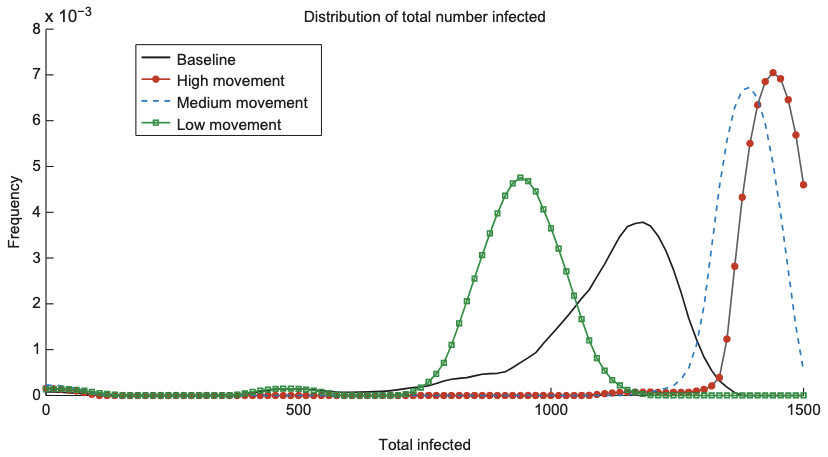
\includegraphics[width=0.8\textwidth]{figures/ch3/manore_1.png}
         \caption{\textbf{Original}}
         \label{fig:validation-1i}
     \end{subfigure}%
     \\
     \begin{subfigure}[b]{\textwidth}
         \centering
         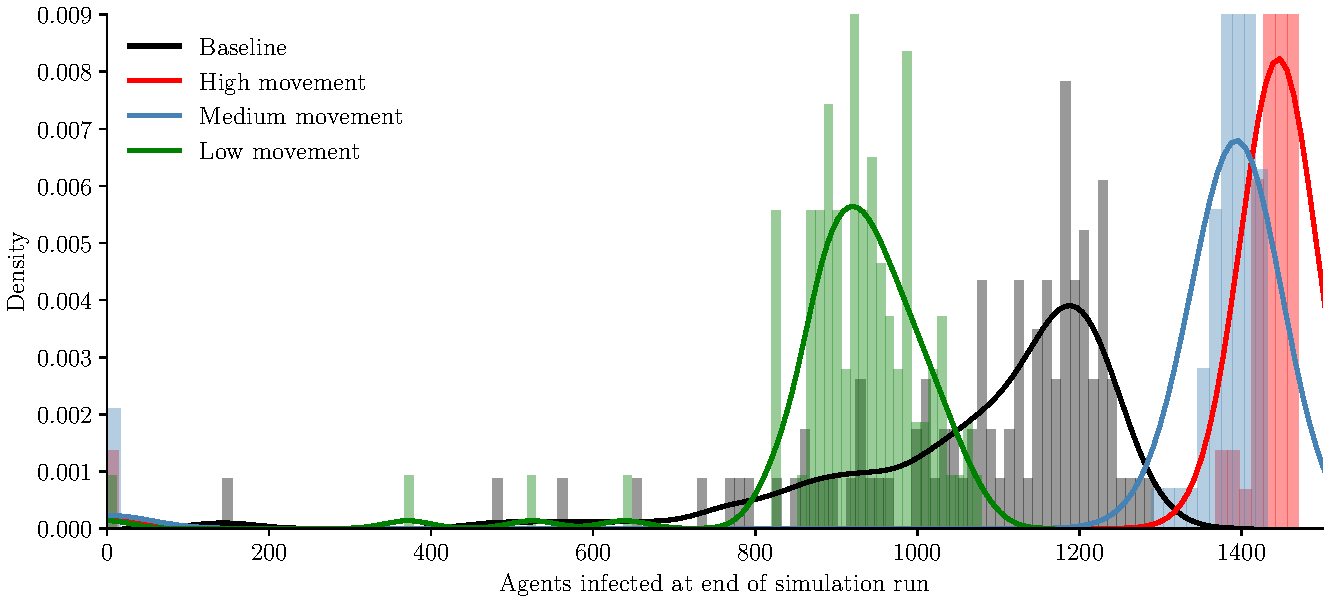
\includegraphics[width=.8\textwidth]{figures/ch3/validation_scaled.pdf}
         \caption{\textbf{Replicated (scaled $y$-axis)}}
         \label{fig:validation-1ii}
     \end{subfigure}%
     \\
     \begin{subfigure}[b]{\textwidth}
         \centering
         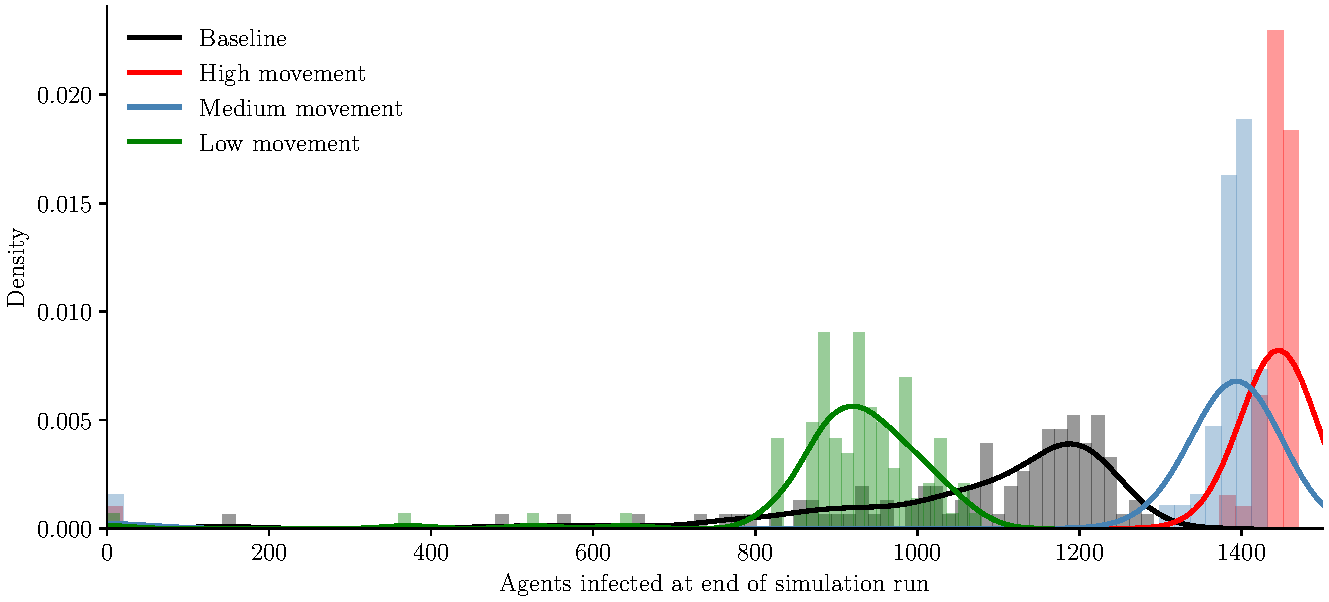
\includegraphics[width=.8\textwidth]{figures/ch3/validation_unscaled.pdf}
         \caption{\textbf{Replicated (unscaled $y$-axis)}}
         \label{fig:validation-1iii}
     \end{subfigure}%
    \bcaption{Distribution of infected agents over simulation for each scenario.}{\textbf{(i)} Results taken from \citet{manore_network-patch_2015} (figure 3 in original paper). \textbf{(ii)} Results from replicated model with the $y$-axis scaled to original figure. \textbf{(iii)} Results from replicated model with unscaled y-axis. Each scenario was run 100 times to mitigate uncertainty from stochasticity.}
    \label{fig:validation-1}
\end{figure}

\begin{figure}[htbp]
     \centering
     \begin{subfigure}[b]{\textwidth}
         \centering
         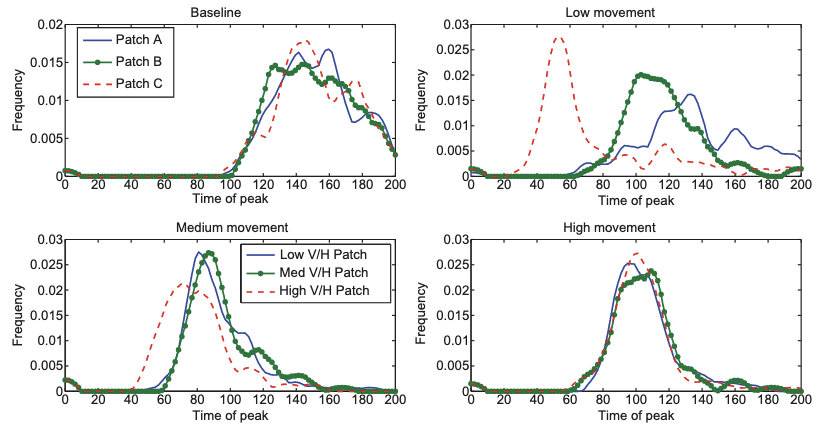
\includegraphics[width=\textwidth]{figures/ch3/manore_2.png}
         \caption{\textbf{Original}}
         \label{fig:validation-2i}
     \end{subfigure}%
     \\
     \begin{subfigure}[b]{\textwidth}
         \centering
         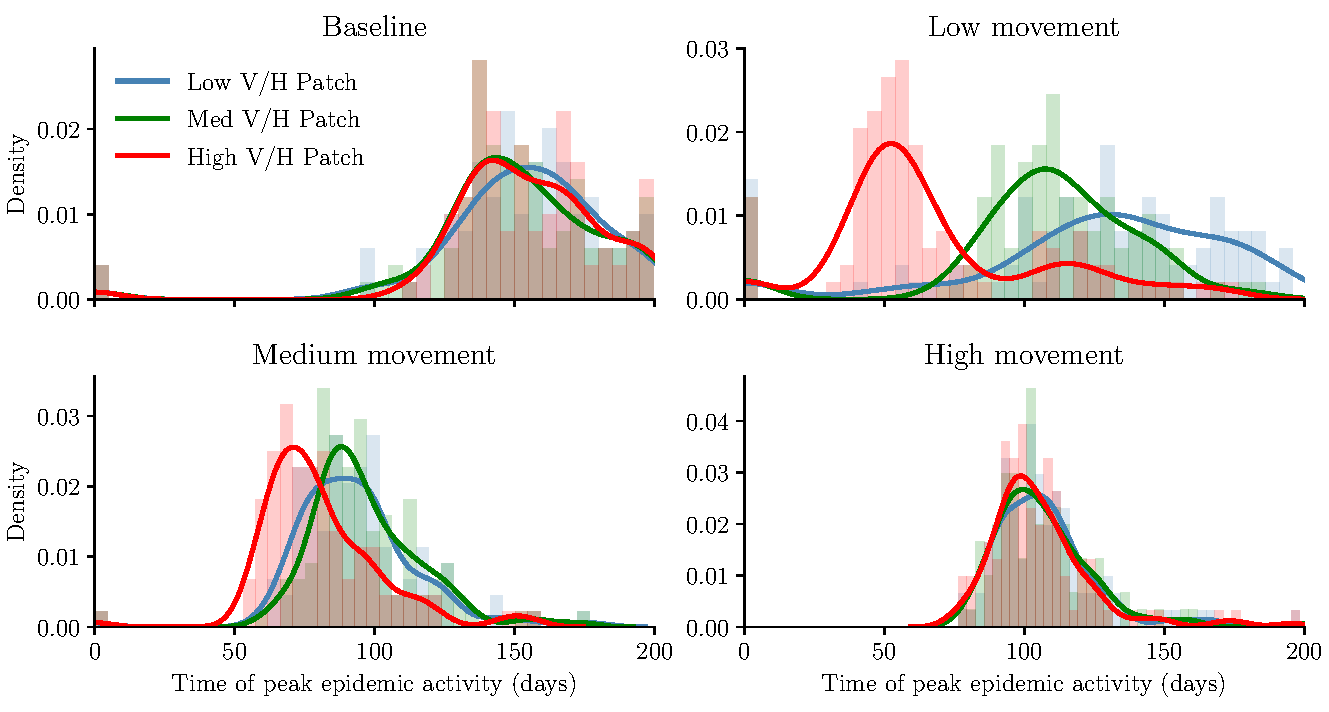
\includegraphics[width=\textwidth]{figures/ch3/validation_2.pdf}
         \caption{\textbf{Replicated}}
         \label{fig:validation-2ii}
     \end{subfigure}%
    \bcaption{Distribution of epidemic peak timings across patches.}{\textbf{(i)} Results taken from \citet{manore_network-patch_2015} (figure 6 in original paper). \textbf{(ii)} Results from replicated model. \q{V/H} means vector-to-host ratio.}
    \label{fig:validation-2}
\end{figure}

\begin{figure}[htbp]
     \centering
     \begin{subfigure}[b]{\textwidth}
         \centering
         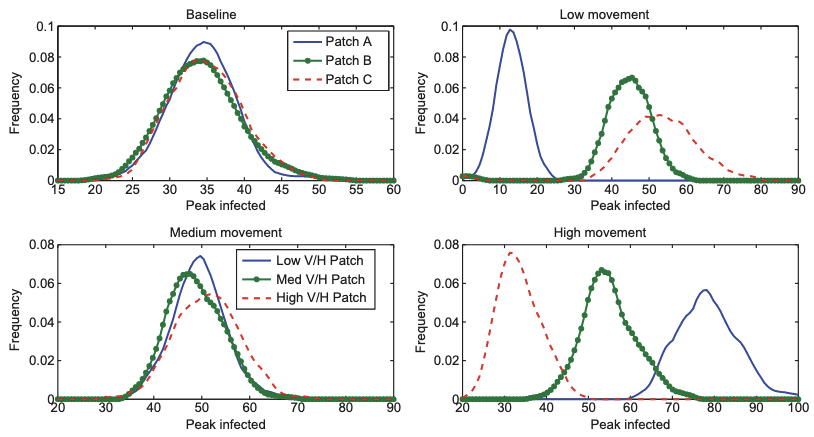
\includegraphics[width=\textwidth]{figures/ch3/manore_3.png}
         \caption{\textbf{Original}}
         \label{fig:validation-3i}
     \end{subfigure}%
     \\
     \begin{subfigure}[b]{\textwidth}
         \centering
         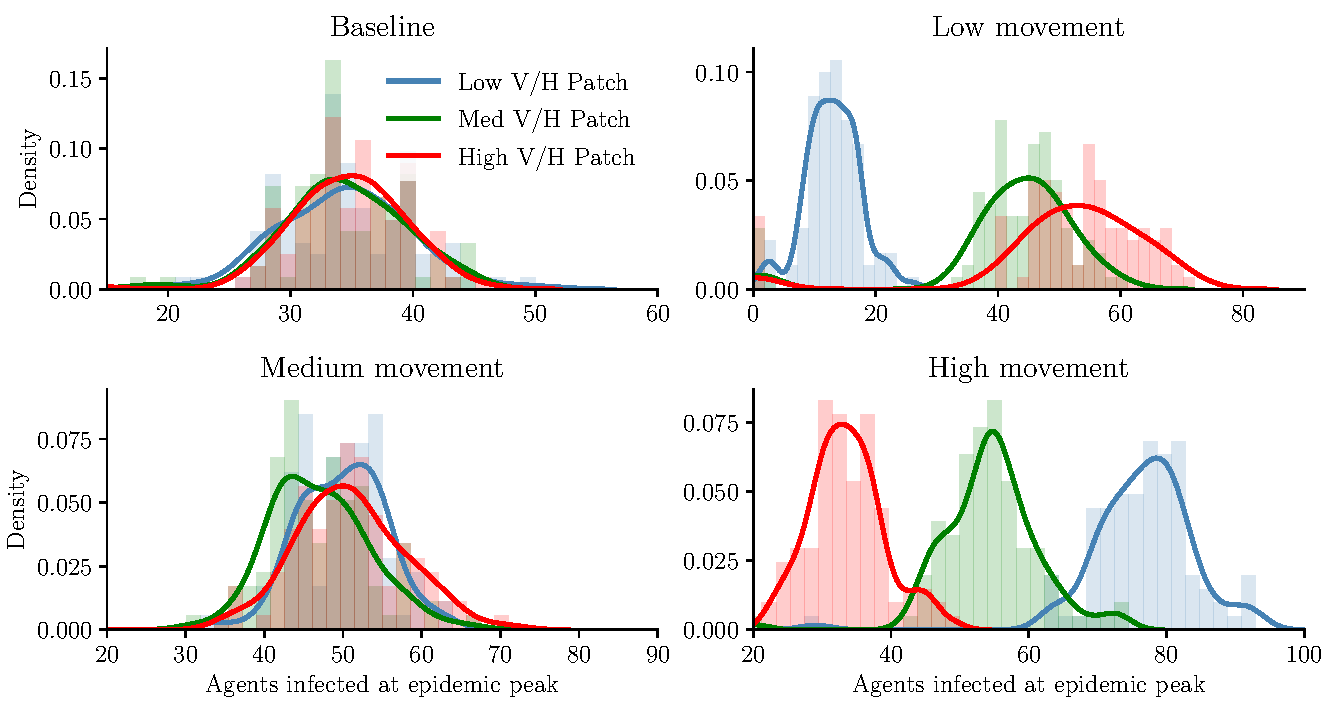
\includegraphics[width=\textwidth]{figures/ch3/validation_3.pdf}
         \caption{\textbf{Replicated}}
         \label{fig:validation-3ii}
     \end{subfigure}%
    \bcaption{Distributions of infected agents during epidemic peaks for each scenario.}{\textbf{(i)} Results taken from \citet{manore_network-patch_2015} (figure 7 in original paper). \textbf{(ii)} Results from replicated model. \q{V/H} means vector-to-host ratio.}
    \label{fig:validation-3}
\end{figure}


\subsection{Validation}

\subsubsection{Results}

Here, I present the findings from the experiments described above and reproduce three figures from \citet{manore_network-patch_2015} to demonstrate the reproduction of the results from the original study with the replicated model. A central finding from the original paper was that heterogeneous patches with medium and high agent movement rates led to higher infection counts over simulations when compared to the baseline scenario. This occurred because in the heterogeneous scenarios, the highest-risk patch (with a mosquito population of $K_v^{(3)}=3750$) was visited more often by agents due to higher movement rates, increasing the spread of infection. The original figure from \citet{manore_network-patch_2015} exhibiting these results is shown in Figure~\ref{fig:validation-1i}, and my own findings in Figure~\ref{fig:validation-1ii} and Figure~\ref{fig:validation-1iii} also demonstrate this relationship\footnote{To align with the original authors, I plot results using kernel density estimation via the Python \textit{seaborn} \cite{waskom_seaborn_2021} library and use the \texttt{kdeplot} function with a smoothing parameter of $\texttt{bw\_adjust}=.55$.}.

As the underlying distributions for Figure~\ref{fig:validation-1i} were not provided in the original paper, I used the scientific imaging software ImageJ \cite{schneider_nih_2012} to estimate peak infection count values from the figure for comparison with the replicated model results. As shown in Table~\ref{tab:peak-alignment}, the absolute relative errors for peak agent infections produced from the replicated model runs compared to the original model across all scenarios were always below 2\%. Overall, this demonstrates the alignment in results of the two models with respect to the maximum total infected agents.

\begin{table}[h]
    \centering
    \begin{adjustbox}{center}
        \begin{tabular}{cccc} \toprule
            {} & \multicolumn{3}{c}{Maximum number of infected agents} \\
            {Scenario} & {Original model (estimated)} & {Replicated model} & {Relative error} \\ \midrule
            Baseline & 1181 & 1189 & 0.68\% \\
            Low movement & 939 & 921& -1.92\% \\
            Medium movement & 1391& 1396& 0.36\% \\
            High movement & 1441& 1447 & 0.42\% \\ \bottomrule
        \end{tabular}
    \end{adjustbox}
    \bcaption{Comparison of maximum infected agents per scenario.}{Original model figures were estimated using ImageJ \cite{schneider_nih_2012}.}
    \label{tab:peak-alignment}
\end{table}

Heterogeneity between patches also explains variation in the timings of peak infections across patches. As results from \citet{manore_network-patch_2015} demonstrate in Figure~\ref{fig:validation-2i}, the highest-risk patch tends to have the earliest peak infections for low and medium movement rates. This is in contrast to the high movement scenario, in which agents traverse the network so thoroughly that infection peaks are roughly equivalent across all the patches. These findings are reiterated in the results from my replicated model shown in Figure~\ref{fig:validation-2ii}.  \\

As \citet{manore_network-patch_2015} observed, there was a trade-off around the risk of a patch (in terms of its vector-to-host ratio) and the accessibility of a patch (in terms of nodes or locations). Figure~\ref{fig:validation-3} highlights how the number of infectious agents during epidemic peaks varied with each experiment scenario. As expected, agents were roughly equally infected in the homogeneous baseline scenario. In the heterogeneous, low movement scenario, since agents with low mobility tended to remain in their patches, the magnitude of infectious agents at epidemic peaks aligned with the risk of each patch. In the high movement scenario, however, this ordering was reversed---when agents have high mobility, they were sufficiently dispersed across all nodes and exposed to infectious forces from all patches. Therefore, the patch with the most locations, and thus agents (the low vector-to-host ratio patch) had the highest number of infectious agents at its epidemic peak.

\subsubsection{Discussion}

The results above convey the alignment of the replicated model with the one described in \citet{manore_network-patch_2015}. First, the reproduced figures demonstrate that the replicated model reproduces the same relationships between salient summary statistics across various scenarios. Second, the reproduced results reiterate the core finding of \citet{manore_network-patch_2015} described in Section~\ref{sec:baseline-model-description} that the model can capture the impacts of heterogeneity on VBD spread. As demonstrated, this is achieved through variation in host mobility patterns and geographical characteristics of environments, which are factors that impact VBD spread in real life \cite{musili_modeling_2024, pepey_mobility_2022}. Ultimately, this validation provides confidence in the replicated model's correctness to be used as a flexible and extendable baseline model.

It should be noted, however, that there are limitations to this model. First, the ODE representation of mosquito populations homogenises mosquito dynamics in patches. As the results for the baseline case demonstrate, when all patches are sufficiently similar, the model resembles well-mixed dynamics, arguably defeating the purpose of the agent-based approach. However, as mentioned, simulating vectors as agents is often computationally infeasible with little data available for informing such a representation \cite{jacintho_agent-based_2010, maneerat_spatial_2016, de_mooij_framework_2023}. Second, VBD spread in the model resembles that of an outbreak, whereas VBDs are often endemic in communities with seasonal variation, particularly in South-East Asia \cite{bhatia_vector-borne_2014}. Despite this, other studies have modelled VBDs as outbreaks \cite{tabares_comparing_2024}, and VBD activity in areas with little to no pre-existing exposure would likely lead to the outbreak patterns reproduced by the model. Finally, exposure during host travel between nodes and patches is not considered in the model, although evidence suggests a high risk of infection during travel \cite{pepey_mobility_2022, sandfort_forest_2020}.

Despite these above limitations, the simplifying assumptions used in this model serve to focus on the dynamics that are relevant to this thesis---preventive behaviours and VBD spread. As \citet{manore_network-patch_2015} highlight themselves, there is a need to \q{adapt ABMs with detailed host activity, behaviour, social, demographic, and geographical data \dots as a step toward creating \dots mitigation strategies.} The following two chapters make progress towards these gaps by parameterising the baseline model to a real-world scenario and extending the ABM with additional features, prior to integrating theories of behaviour change.